\documentclass{abnt}
\usepackage[utf8]{inputenc}
\usepackage[english,brazilian]{babel}
\usepackage{hyperref}
\usepackage{url}
\usepackage{indentfirst}
\usepackage{blindtext}
\hypersetup{%
    pdfborder = {0 0 0}
}
\usepackage{graphicx}
\graphicspath{{./imagens/}}
\usepackage{placeins}

\begin{document}

\autor{Rafael Tavares Amorim \\ Juliano Rodovalho Macedo \\ Wolmir L. F. Nemitz}

\titulo{Entrega 3: Gestão de Disponibilidade \\ Versão 2.0}

\instituicao{Universidade Federal do Pampa \par Engenharia da Software \par Resolução de Problemas V}

\local{Alegrete - Rio Grande do Sul, Brasil}

\data{15 de Setembro de 2012}

\capa

\folhaderosto

\tableofcontents

\listoffigures


\chapter{INTRODUÇÃO}

	Este relatório tem por finalidade apresentar a fundamentação teórica e tecnológica utilizada no terceiro \emph{sprint}, o nosso Product Backlog completo e atualizado, 
	o Sprint Backlog munido de nossas especificações de engenharia juntamente com o detalhamento da solução, e por fim,o link de referência visando o acesso ao sistema.


	
	\section{Metodologia Ágil}
	
		Metodologia ágil é um famoso conjunto de metodologias de desenvolvimento de software, 
		com foco na mitigação dos riscos, esta metodologia aposta em pequenos ciclos iterativos de desenvolvimento de software,
		onde ocorre a repetição de cada tarefa comum em um processo de software, ou seja, em cada ciclo realiza-se analise, projeto,
		implementação e testes, referentes aquele módulo, desta forma busca-se à capacidade real de implantar um nova versão 
		do sistema ao final de cada ciclo; Antes de iniciar-se uma nova iteração a equipe responsável por todo o projeto é reunida 
		e reavalia-se as características, metas e prioridades do projeto como um todo, para que estas sejam aplicadas no próximo ciclo.
		
		Os modelos ágeis são hoje a principal alternativa as metodologias tradicionais de desenvolvimento de software, 
		as quais apresentam diversos problemas estruturais que comprometem a maioria dos projetos, 
		baseados nas necessidades atuais do mercado de software.
	
	\section{Scrum}
	
		\subsection{Visão Geral}
		
			O \emph{scrum} é uma metodologia ágil de desenvolvimento de software, embora muitos consideram-no como um framework ágil, 
			o seus maior objetivo é agilizar o processo de desenvolvimento de software com pequenas entregas ao cliente de forma iterativa
			visando agregar-se valor ao produto a cada ciclo(iteração) . Em sua existem três papéis neste processo, são eles: \emph{Product Owner, Scrum Master, Team}.
		
		\subsection{Papéis}
		
			O \emph{Product Owner} é um papel muito importante no \emph{scrum}, cabe a ele definir quais funcionalidades devem ou
			não existir no sistema por meio de \emph{user stories} e também definir a prioridade delas. Este pa\texttt{}pel também
			trata de aprovar ou rejeitar o trabalho realizado e dizer se foi realizado como esperado.
			
			O \emph{scrum master} tem papel de manter a produtividade da equipe, facilitando o processo de \emph{scrum} e resolver impedimentos
			no decorrer do \emph{sprint}. Ele ajuda o time a se manter organizado e certificar que as regras do processo estão sendo
			seguidas corretamente. O \emph{scrum master} não dita o que o time deve fazer mas sim ajuda o time se manter autônomo,
			organizado e com uma boa produtividade. 
			
			O \emph{team} tem papel de transformar os itens de \emph{backlog} em produtos que serão entregues de forma incremental em cada
			sprint. Cabe ao time ter autonomia própria para se organizar e trabalhar de forma de colaborativa ajudando uns aos
			outros sem a necessidade de existência de um "chefe" para dizer o que deve ser feito.
		
		\subsection{Processo}
		
			O processo de \emph{scrum} é trabalhado em cima de vários ciclos chamados de \emph{sprint}, que possuem um tempo fixo, geralmente de
			1 a 4 semanas. Para cada \emph{sprint} é realizado a escolha de \emph{user stories} que estão no \emph{product backlog}. No \emph{product backlog} temos uma lista priorizada 
			pelo \emph{product owner} das funcionalidades desejadas do projeto, e parte desta lista irá forma o \emph{sprint backlog}. É uma coleção de \emph{user stories}.
			
			Em um ciclo, o time irá realizar o \emph{sprint backlog} que contêm os itens de \emph{backlog} que o time concordou 
			completar em um ciclo de \emph{sprint}, cada item de \emph{backlog} é quebrado em tarefas, atribuídas para equipe e estimado o tempo de realização.
			
					
			O \emph{backlog item} ou também conhecido como \emph{user story} é um recurso/funcionalidade desejada no sistema que vão compor o
			\emph{product backlog}. Uma \emph{user story} usualmente é composta por um ator do sistema e a ação para alcançar determinado
			objetivo. Exemplos: 
				\begin{itemize}
					\item Como um <usuário> Eu posso <realizar ação> para alcançar <determinado objetivo>
					\item Como um cliente, eu posso criar um perfil no sistema
					\item Como um cliente, eu posso escolher um usuário e senha
					\item Como um administrador, eu posso bloquear contas de clientes
				\end{itemize}
					 
					
			No \emph{sprint planning}, a equipe decidirá quais \emph{backlog itens} irão para o \emph{sprint backlog}. Depois da priorização das \emph{user
			stories} pelo \emph{product owner}, a equipe seleciona o item do topo do \emph{product backlog}, o qual tem maior prioridade, para a
			discussão e criação das tarefas necessárias para entrega do item. Então as tarefas são atribuídas e estimadas em
			tempo, este processo é repetido até que o time decida que não há possibilidade de realização de mais itens.
			
			Com a ajuda do\emph{Burndown} que é um gráfico que oferece uma forma poderosa que podemos analisar o andamento do projeto. Podemos estimar a velocidade de andamento do time, atrasos e tempo de 
			execução de cada \emph{user story}.
			
			Por meio de um reunião diariamente, podemos também verificar impedimentos que podem afetar a produtividade da equipe, conhecida como \emph{daily meeting}, 
			é uma reunião com duração aproximada de 15 minutos,	conduzida pelo \emph{scrum master} e tem como foco 3 perguntas para todo membro da equipe:
				\begin{itemize}
					\item O que eu fiz ontem?
					\item O que eu estou fazendo hoje?
					\item O que está me impedindo de fazer?
				\end{itemize}
			
			Apesar da reunião ser conduzida pelo scrum master, cada membro deve responder para o time inteiro e não somente para o
			\emph{scrum master}, todos devem estar de pé na reunião e falar somente quando for perguntado pelo \emph{scrum master}. No final da
			reunião é discutido por todos soluções caso haja algum impedimento.
			
			No final de um \emph{sprint}, ocorre uma reunião informal, chamada \emph{sprint review} que tem intuito de demonstrar o que foi 
			realizado no sprint com a presença da equipe, \emph{scrum master}, \emph{product owner} e stakeholders. Também é feita a reunião chamada \emph{sprint retrospective}
			que é uma reunião da equipe que tem objetivo de discutir se o \emph{sprint} foi realizado com sucesso ou se é necessário melhorias.
			
			Um projeto em \emph{scrum} pode ser parado a qualquer momento, as vezes o cliente percebe que as funcionalidade implementadas já foram
			suficientes e atendem a necessidade atual assim não dispersando dinheiro em funcionalidade que talvez nunca seriam utilizadas.
			
			As informações desta seção foram retiradas da referência \cite{SCRUMEPF}.
	
	\section{Python}
	
		\emph{Python} é uma conceituada linguagem de programação de alto nível, interpretada, orientada a objetos e de tipagem forte. 
		Idealizada como uma linguagem que valorize o tempo e esforço do programador, Python foca a legibilidade do código,
		 sua indentação, velocidade de desenvolvimento e expressividade. Dentro desta filosofia podemos destacar a forte indentação da linguagem e sua sintaxe simples , 
		 o que facilita a leitura melhorando o visual organizacional da linguagem, este aspecto limpo e coerente coopera para um rápido aprendizado.\cite{PYTHON}
	
	\section{Pip}
	
		Devido à grande quantidade de extensões, bibliotecas e frameworks que utilizam \emph{Python}, a comunidade desta linguagem criou um repositório centralizado de pacotes, o \emph{Python Package Index}.
		\emph{Pip} é uma ferramenta para instalar e gerenciar pacotes \emph{Python}, tais como aqueles encontrados no \emph{Python Package Index}.\cite{PIPSITE}

	\section{Django}
		\emph{Django} é um framework para desenvolvimento web em Python, cuja proposta
		é encorajar a construção rápida e pragmática de aplicações.\cite{DJANGOSITE}
		O \emph{django} segue a arquitetura model-view-controller. O modelo das aplicações
		é definido através de classes de modelo que serão mapeadas, mediante o lançamento do projeto,
		para entidades relacionais no banco de dados definido pelos desenvolvedores. A \emph{view} é
		representada através de funções ou métodos que processam requisições com um sistema
		de \emph{templates}. O \emph{controller} é nada mais que a customização das URLs da aplicação,
		que podem ser detectadas através de expressões regulares e redirecionam o
		usuário à \emph{view} apropriada.\cite{DJANGOWIKIPEDIA}
	
	\section{South}
		\emph{South} é uma ferramenta de migração de dados em aplicações \emph{Django}, 
		permite ao desenvolvedor migrar as informações do banco de dados apos refatorações no modelo
		sem á real necessidade em manipular-se o banco, executando as alterações necessárias 
		no mesmo de acordo com as modificações realizadas.
				
		Suas principais característica são: 
			\begin{itemize}
			\item Criação e migração automática: \emph{South} é possível visualizar o que realmente foi modificado em seu arquivo models.py
			 e automaticamente escrever a migrações que corresponda as estas alterações.
			\item Independência de banco de dados: Em questões gerais, o \emph{South} é independente da tecnologia utilizada no banco de dados, 
			suportando atualmente os cinco \emph{backends} de bancos de dados mais conceituados no mercado.
			\item Avançado: \emph{South} reconhece e trabalha com o conceito de aplicativos \emph{Django}, permitindo que o desenvolvedor configure 
			suas migrações para aquelas aplicações escolhidas, e permite ao mesmo trabalhar sobre \emph{syncdb} nas demais.
			\end{itemize}
			
		As informações desta seção foram retiradas da referência \cite{SOUTH}.
	
	\section{Jenkins}
			
				\emph{Jenkins} é um servidor de integração contínua, de código fonte aberto e escrito em Java, disponibiliza mais de 300 plugins 
				com suporte aos mais diversos tipos de desenvolvimento de software. O \emph{Jenkins} prover todo o processo de integração 
				contínua durante o desenvolvimento de software.
				
				O processo de integração contínua visa melhorar a qualidade do produto de software entregue em cada versão, reduzindo o tempo efetivo de integração,
				substituindo então as práticas tradicionais de aplicação do controle de qualidade após o desenvolvimento completo. Os princípios da
				integração contínua são:
				\begin{itemize}
				  \item Manter o código fonte em um repositório de controle de versão;
				  \item Automatizar a construção de software;
				  \item Fazer a construção da software e testa-lo automaticamente;
				  \item Todos os desenvolvedores devem submeter\emph{(commitar)} para a mesma base de repositório diariamente;
				  \item Toda submissão para o repositório base deve ser construído;
				  \item A construção deve ocorrer rapidamente visando identificar os problemas o mais breve possível;
				  \item Testar em um ambiente clone de produção\emph{(simular o ambiente real)};
				  \item Deixar sempre a última construção bem sucedida disponível para os \emph{stakeholders} e testadores;
				  \item Todos podem ver o resultado das últimas construções;
				  \item Automatizar o \emph{deploy};
				\end{itemize}
				
				O momento de testes, durante o deploy é de extrema importância para obter-se bons resultados com a integração contínua. Existem 
				diversos mecanismos implementados em varias linguagens que podem não somente testar o funcionamento total da aplicação mas 
				também verificar a qualidade do código fonte escrito, utilizando para isso fatores como padrão de codificação, detecção de cópias, 
				detecção de erros em sintaxe e problemas de lógica, comumente chamado de inspeção contínua.
				
				A ferramenta \emph{Jenkins} entra para a execução do processo de integração contínua, irá tratar de obter o código fonte,
				realizar a construção com ajuda do \emph{Maven}\cite{MAVENBUILDTOOL} ou \emph{Ant}\cite{ANTBUILDTOOL}, realizar a execução dos testes 
				e fazer o deploy para o servidor.\cite{JENKINS-BUILD}

		\section{Klaros Testmanagement}
		
			É uma aplicação web baseada em AJAX e escrita em Java, seu intuito é melhorar a organização e gerenciamento do processo de teste como um todo. 
			O sistema permite a construção dos casos de teste, gerencia-los, dividi-los em suítes de testes, cadastrar os
			ambientes de teste(sistema/ambiente onde os testes serão rodados), executar os testes e coletar seus resultados.
			
			Através dos testes realizados no sistema, podemos construir os casos de teste, estes são nomeados, 
			descritos (descrição, pré-condição e pós-condição), priorizados entre os demais, possuem estado de execução, 
			modo de execução e podem ser divididos em vários passos. Também é possível definir-se o ambiente de execução, 
			como o Sistema Operacional ou Navegador para aplicações Web. O software apresenta uma interface relativamente amigável, 
			embora seu mapeamento e feedbacks não sejam muito claros, isso não afeta no modo globalmente na utilização da ferramenta.
			
			\begin{itemize}
			  \item Possui versionamento e histórico sobre os dados.
			  \item Trabalha com casos de teste e seus resultados.
			  \item Gera relatórios em gráficos e tabela sobre os testes. Podendo ser exportado em vários formatos como PDF, HTML, XML, entre outros.
			  \item Possui suporte a integração com ferramentas de gerenciamento de projeto como: \emph{Redmine, Jira, Trac e Bugzilla}.
			  \item É possível através de plugins dos sistemas de integração continua (\emph{Hudson/Jenkins}) importar os relatórios de
			  execução dos testes automatizados.
			  \item Pode ser instalado em Windows por meio de um executável e Linux por meio de um arquivo jar.
			\end{itemize}
			
			A ferramenta apresentou ótimo desempenho, auxiliando de modo global dentro dos testes realizados no sistema, 
			seus recursos agregaram expressivo valor aos resultados colhidos em cada teste, destaque para seus relatórios 
			os quais apresentam excelente corpo de informações, como gráficos, tabelas e detalhamento de cada ocorrência 
			durante a execução dos teste. Sua integração com o sistema de gerenciamento de defeitos é feito na parte administrativa do software, 
			onde informa-se o endereço, usuário e senha, para então realizar-se a integração.
			
			O embasamento teórico para as informações contidas nesta seção podem ser encontradas na referência \cite{KLAROS}.
			
	\section{MySQL}

		\emph{MySQL} é um famoso sistema de gerenciamento de base de dados, conta com diversas funcionalidades e sua fácil abordagem foi o motivo chave para sua escolha.
		É o \emph{SGBD} utilizado no projeto de gerenciamento de disponibilidades por ser livre de custos e amplamente documentado.\cite{MYSQLWIKI}
	
\clearpage

\chapter{SPRINT}
	
		Esta seção aborda as informações sobre o Sprint III, demonstrando o nosso \emph{Sprint Backlog} logo a baixo. Os diagramas de casos de uso e classes para cada \emph{User Story} está disponível nas seções seguintes.
	
	\section{Detalhamento da Solução}
	
		Após a apresentação do problema proposto a equipe trabalhou sobre as propostas de solução que melhor envolviam o ambiente já definido no \emph{sprint} anterior,
		apos este levantamento determinou-se que o projeto seria construído sobre os seguintes pilares:
		\begin{itemize}
		\item  A linguagem de programação \emph{Python}.
		\item O ambiente de desenvolvimento integrado com \emph{Aptana Studio 3}.
		\item O ambiente de desenvolvimento Web.
		\item  O framework de desenvolvimento \emph{Django}.
		\item  A ferramenta de gerenciamento \emph{Redmine}.
		\item  A ferramenta de versionamento \emph{GitHub}.
		\item  A ferramenta de gerenciamento e execução de testes \emph{Klaros}.
		\item  A ferramenta de integração contínua \emph{Jenkins}.
		\end{itemize}
		
		\subsection{Funcionalidades - Versão 2.0}
		
		As funcionalidades entregues nesta versão são:
		
			\begin{itemize} 
			\item Crud de Compromissos:
			\subitem Informar a frequência de repetição do compromisso
			\subitem Dias da semana para a repetição do compromisso
			\subitem Fim da repetição do compromisso
			
			\item Crud de Área de Formação:
			\subitem Informar área de formação
			\subitem Visualizar área de formação
			\subitem Remover área de formação
			
			\item Crud Disciplinas de Preferência:
			\subitem Informar disciplinas de preferência
			\subitem Visualizar disciplinas de preferência
			\subitem Editar disciplinas de preferência
			\subitem Remover disciplinas de preferência
			
			\item Crud Grade de Aulas:
			\subitem Visualizar grade de aulas
			
			\item Crud Disponibilidade Horária para Aulas:
			\subitem Informar disponibilidade de horário para ministrar aulas
			\subitem Visualizar disponibilidade de horário para ministrar aulas
			\subitem Remover disponibilidade de horário para ministrar aulas
			
			\end{itemize}
			
	\clearpage
	\section{User Story 1}
	
		\begin{itemize}
			\item Como professor, eu quero informar os dias que estarei na Unipampa para que os outros possam me encontrar para assuntos urgentes.
		\end{itemize}
				
		\begin{figure}[h]
			\begin{center}
				 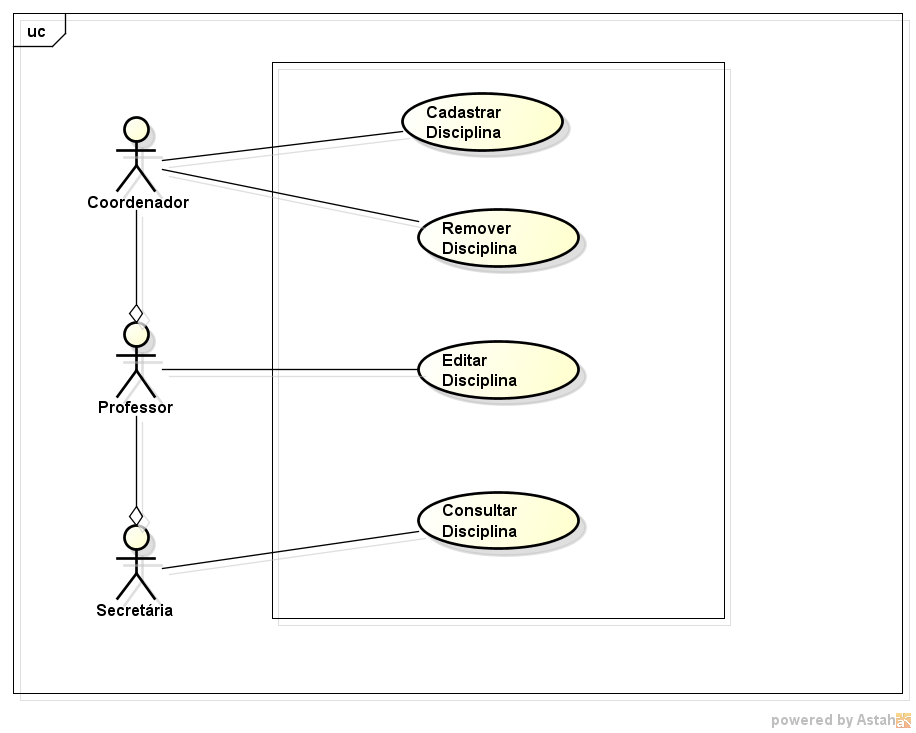
\includegraphics[width=400px]{casoUsoDisciplinas}
				 \caption{Diagrama de Caso de Uso - Cadastro de Disciplinas}
				 \label{fig:casoUsoCadastroDisciplina}
			\end{center}
		\end{figure}
		\FloatBarrier
	
	\clearpage	
	\section{User Story 2}

		\begin{itemize}
			\item Como professor, eu quero informar meu horário disponível para as aulas, [Transferido para a Semana 03 (minhas disciplinas de preferência 
			e área de formação para que o coordenador possa montar a grade de aulas de acordo com os dados que informei)].
		\end{itemize}
			
	
		\begin{figure}[h]
			\begin{center}
				 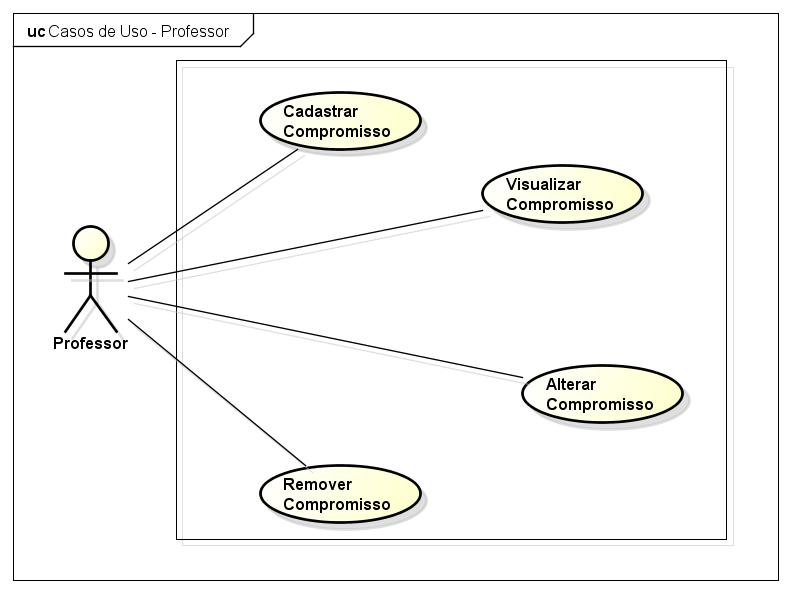
\includegraphics[width=400px]{casoUsoProfessor}
				 \caption{Diagrama de Caso de Uso - Agenda do Professor}
				 \label{fig:casoUsoAgendaProfessor}
			\end{center}
		\end{figure}
		\FloatBarrier
	\clearpage
	\section{User Story 3}

		\begin{itemize}
			\item Como professor, eu quero visualizar minha grade horária de aulas para saber os horários que tenho que dar aula.
			[Adicionado a Semana 03 (Como professor, eu quero informar minhas disciplinas de preferência e área de formação para que o coordenador 
			possa montar a grade de aulas de acordo com os dados que informei.)].
		\end{itemize}
	
		
		\begin{figure}[h]
			\begin{center}
				 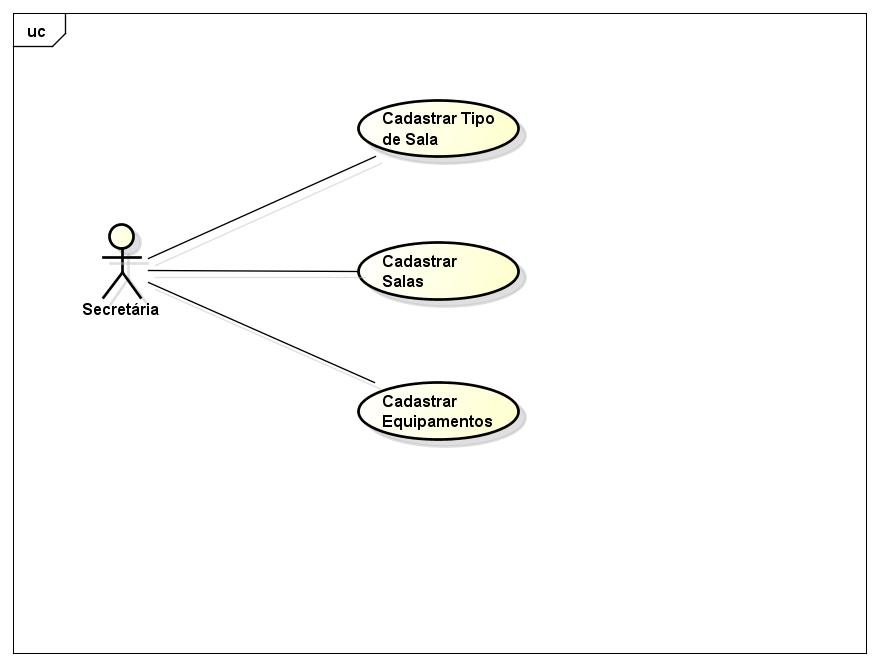
\includegraphics[width=400px]{casoUsoSecretaria}
				 \caption{Diagrama de Caso de Uso - Secretaria}
				 \label{fig:casoUsoSecretaria}
			\end{center}
		\end{figure}
		\FloatBarrier
		
	\clearpage
	\section{Diagrama de Classes}
		
		O figura \ref{fig:diagramaClassesModelo} mostra o diagrama de classes da solução implementada para as \emph{user stories} do \emph{sprint}.
	
		\begin{figure}[h]
			\begin{center}
				 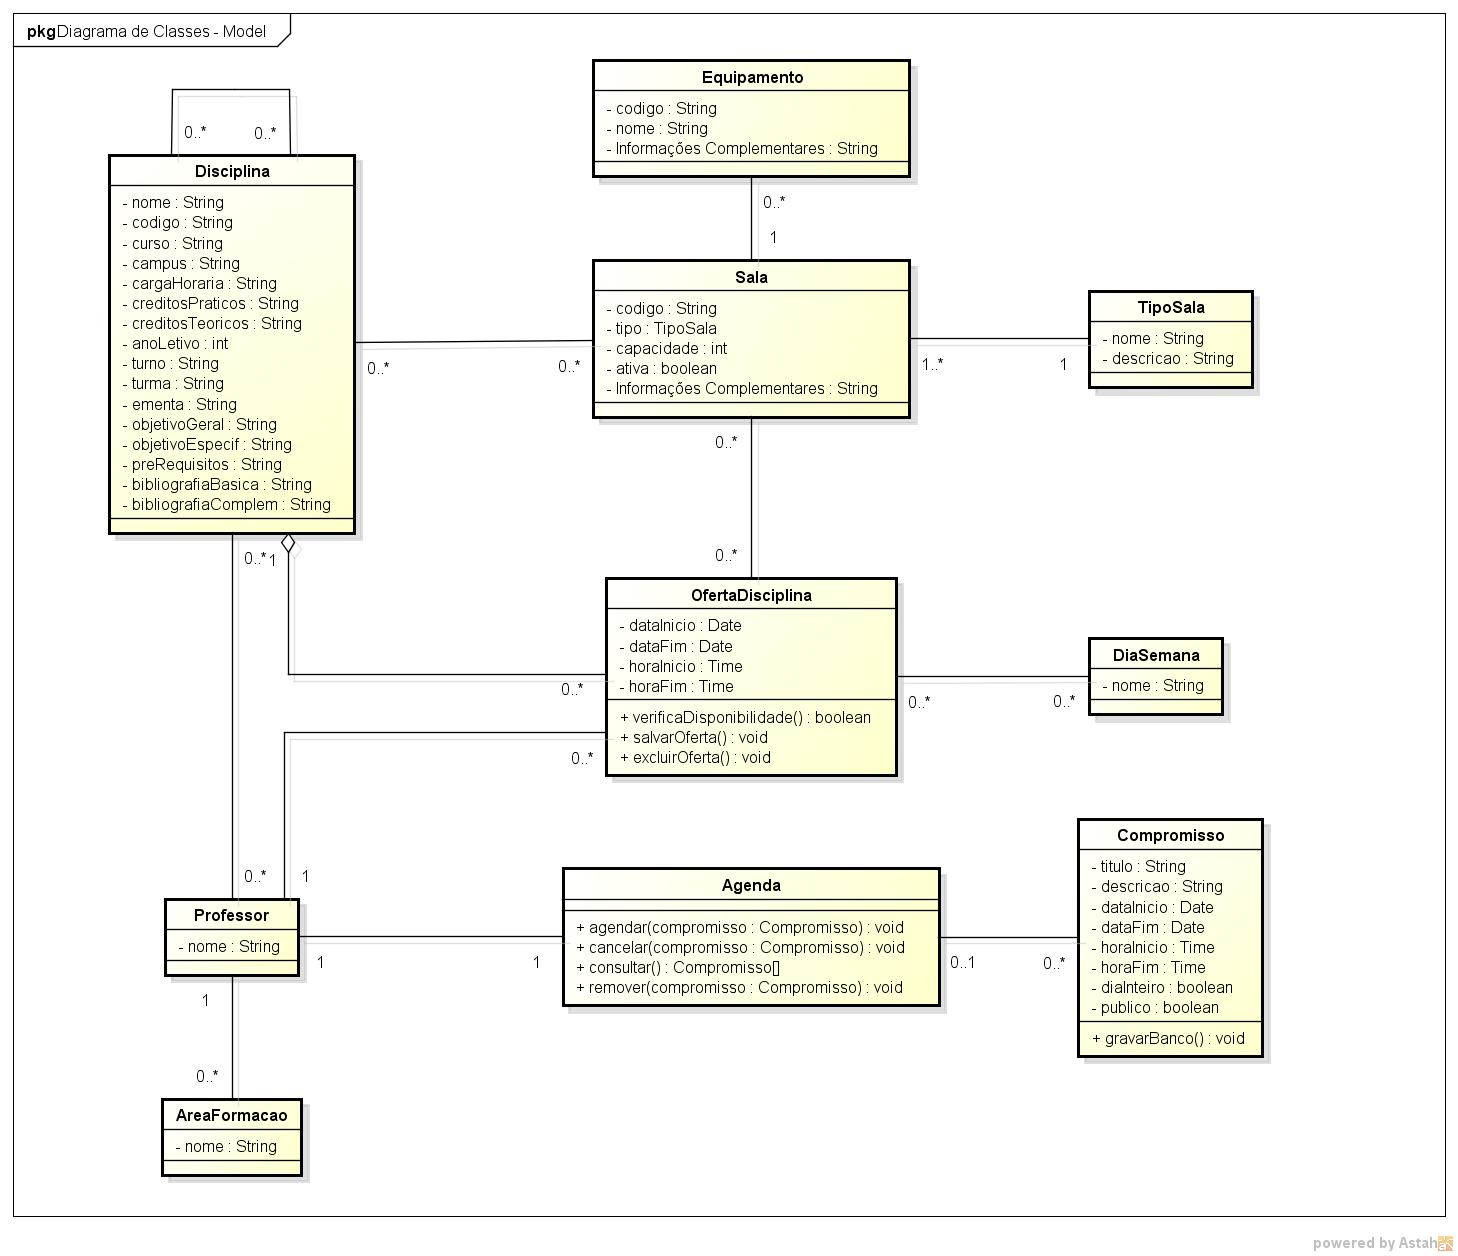
\includegraphics[width=400px]{classesmodelo}
				 \caption{Diagrama de Classes Modelo}
				 \label{fig:diagramaClassesModelo}
			\end{center}
		\end{figure}
		\FloatBarrier

	\clearpage

	\section{Acesso ao Sistema}
			De acordo com o planejamento construído no \emph{sprint} anterior o qual definimos nossa infraestrutura de desenvolvimento, 
			o sistema esta em integração contínua com o servidor de testes on-line, podendo ser acessado a partir da seguinte url:
		
			\url{http://chicago1.vsnetwork.net/}
			

	\section{Acesso às Ferramentas}
		
		O gestor de projeto pode ser acessado através da url: \url{http://redmine.vsnetwork.net/projects/rp-v} , o qual está visivelmente público em todas as atividades do projeto. 
		
		O código fonte do projeto pode ser acessado pelo github\cite{GITHUB} na url: \url{https://github.com/dextervip/rpv}. 
		
		As construções automatizadas do jenkins podem ser acessadas pela url: \url{http://chicago2.vsnetwork.net:8080/job/RPV}.

	\clearpage

	%Referências Bibliograficas
	\nocite{*}
	\bibliographystyle{abnt-num}
	%\bibliographystyle{plain}		
	\bibliography{bibliografia}		

\end{document}